\documentclass[german=false,thesistype=bachelor,proposal]{tubsthesis}

\usepackage{lipsum}
\usepackage{pgfgantt} % Schedule

\thesisname{Johanna Doe}
\thesismatrikel{1234567}
\thesisemail{j.doe@tu-braunschweig.de}
\thesismajor{Informatik}
\thesisduration{3}
\thesissupervisors{Super Visor, M. Sc.}{Dr. Dipper Visor}{}
\thesisprofessor[Prof.\,Dr.-Ing.\,Jane Smith]{Prof.\,Dr.-Ing.\,Lars Eisbär}
\thesistitle{Titel der Thesis}{Title of the thesis}
\thesisbegindate{2020-01-01}
%\thesisenddate{2020-01-02}
\thesispresentationpoints{5.7}

\addbibresource{bibliography.bib}

\thesisinstitute{Institute of Perfect Writing in IT}

\begin{document}
\begin{thesis}

\chapter{Introduction and Motivation}
\lipsum

\chapter{Related Work}
\lipsum[1-3]

\begin{figure}
\centering
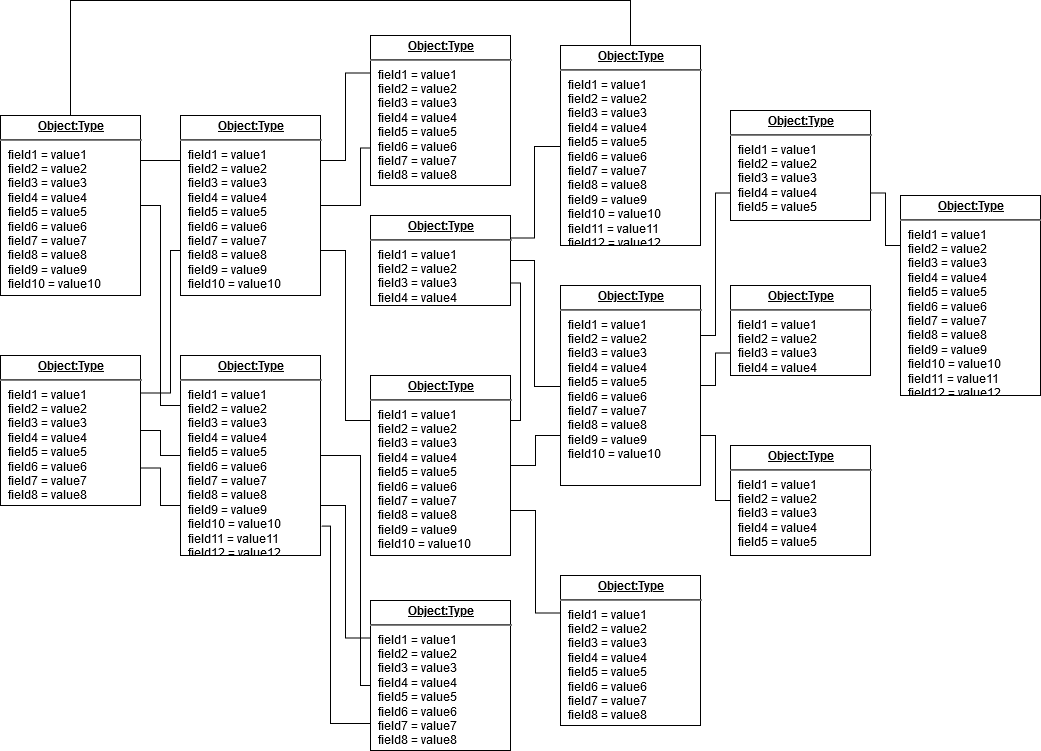
\includegraphics[width=\textwidth]{images/example_diagram.png}
\caption{Some diagram, not relevant to anything~\cite{lisa}}
\label{fig:inga}
\end{figure}

\lipsum[4-5]

\chapter{Task}
\lipsum[1-3]

\chapter{Evaluation}
\lipsum[1-4]

\newpage
\chapter{Schedule}

% für Masterarbeiten / for Master's Theses
For Master's Theses:\\
\begin{ganttchart}[hgrid, vgrid,]{1}{24}
\gantttitle{Week}{24} \\
\gantttitlelist{1,...,24}{1} \\
\ganttbar{WP1}{1}{4} \\
\ganttbar{WP2}{5}{9} \\
\ganttmilestone{Milestone}{6} \\ % Meilenstein nach 6 Wochen / milestone after 6 weeks
\ganttmilestone{Intermediate presentation}{6} \\ % Zwischenvortrag nur bei Masterarbeiten / intermediate presentation only for Master's Theses
\ganttbar{WP3}{7}{17} \\
\ganttbar{WP4}{18}{23} \\
\ganttbar{Print and turn in}{24}{24} \\
\ganttmilestone{Final presentation}{24}
\end{ganttchart}

% für Bachelorarbeiten / for Bachelor's Theses
For Bachelor's Theses:\\
\begin{ganttchart}[hgrid, vgrid,]{1}{12}
\gantttitle{Week}{12} \\
\gantttitlelist{1,...,12}{1} \\
\ganttbar{WP1}{1}{4} \\
\ganttbar{WP2}{5}{9} \\
\ganttbar{WP3}{7}{11} \\
\ganttbar{Print and turn in}{12}{12} \\
\ganttmilestone{Final presentation}{12}
\end{ganttchart}

\section{Work Packages}
% Jedes Arbeitspaket wird genau beschrieben.
% Jedes Arbeitspaket bekommt eine stichpunktartige Liste von Muss- und Kann-Kriterien,
% deren Erfüllung später überprüfbar ist.

Each work package is described precisely.
Each work packages has a bullet point list of mandatory and optional criteria
that can be verified later.
\lipsum[4]

\subsection{WP1: ...}
\lipsum[1]

\subsection{WP2: ...}
\lipsum[2]

\subsection{WP3: ...}
\lipsum[3]

\section{Milestones}
% nur bei Masterarbeiten
% Hier wird aufgelistet, welche Kriterien bis zum Meilenstein erfüllt sein müssen.
% Für Arbeitspakete die über den Meilenstein hinaus gehen (hier etwa AP2) müssen die Kriterien
% genau beschrieben sein, die am Meilenstein erfüllt sind.

only for Master's Theses
Please list here, which criteria have to be fulfilled until the milestone is reached.
For work packages that outlast the milestone (here WP2) the criteria,
that will be fulfilled at the milestone, have to be described precisely.

\lipsum[5]

\end{thesis}
\end{document}